\documentclass[a4paper,12pt]{article}
\usepackage[utf8]{inputenc}
\usepackage{amsmath}
\usepackage{amsfonts}
\usepackage{amssymb}
\usepackage{graphicx}
\usepackage{braket}

\numberwithin{equation}{section}
\renewcommand\thesubsection{\alph{subsection}}
\newcommand{\bvp}[1]{\mathbf{#1}'}
\newcommand{\bv}[1]{\mathbf{#1}}

%opening
\title{Quantum II HW2}
\author{Vincent Baker}

\begin{document}

\maketitle

\section{Problem 1}

Electronic configurations of \\
a. He(Z=2) $1s^2$ \\
b. Ne(Z=10) $1s^2 2s^2 2p^6$\\
c. Ar(Z=18) $1s^2 2s^2 2p^6 3s^2 3p^6$ \\
d. O (Z=8) $1s^2 2s^2 2p^4$ \\
e. Fe (Z=26) $1s^2 2s^2 2p^6 3s^2 3p^6 4s^2 3d^6 $\\

\section{Problem 2}
Nuclear configuration of:\\
a) $^4_2He$: Protons(2):$1s_{1/2}^{(2)}$  Neutrons(2): $1s_{1/2}^{(2)}$ \\
b) $^{16}_8O$: Protons(8): $1s_{1/2}^{(2)}\ 1p_{3/2}^{(4)}\ 1p_{1/2}^{(2)}$  Neutrons(8): $1s_{1/2}^{(2)}\ 1p_{3/2}^{(4)}\ 1p_{1/2}^{(2)}$ \\
c) $^{40}_{20}Ca$ Protons (20): $1s_{1/2}^{(2)}\ 1p_{3/2}^{(4)}\ 1p_{1/2}^{(2)}\ 1d_{5/2}^{(6)}\ 2s_{1/2}^{(2)}\ 1d_{3/2}^{(4)} $  
\\ Neutrons (20):$1s_{1/2}^{(2)}\ 1p_{3/2}^{(4)}\ 1p_{1/2}^{(2)}\ 1d_{5/2}^{(6)}\ 2s_{1/2}^{(2)}\ 1d_{3/2}^{(4)} $ \\
d) $^{56}_{26}Fe$ Protons (26): $1s_{1/2}^{(2)}\ 1p_{3/2}^{(4)}\ 1p_{1/2}^{(2)}\ 1d_{5/2}^{(6)}\ 2s_{1/2}^{(2)}\ 1d_{3/2}^{(4)}\ 1f_{7/2}^{(6)} $  
   \\ Neutrons (30): $1s_{1/2}^{(2)}\ 1p_{3/2}^{(4)}\ 1p_{1/2}^{(2)}\ 1d_{5/2}^{(6)}\ 2s_{1/2}^{(2)}\ 1d_{3/2}^{(4)}\ 1f_{7/2}^{(8)}\ 2p_{3/2}^{(2)} $\\
e) $^{13}_6Ca $ Protons (6): $1s_{1/2}^{(2)}\ 1p_{3/2}^{(4)} $ Neutrons (7): $1s_{1/2}^{(2)}\ 1p_{3/2}^{(4)}\ 1p_{1/2}^{(1)} $

\section{Problem 3}
The ground state configurations for the three atoms are:\\
a) $^{57}_{26}Fe$: Protons (26) valence $1f_{7/2}^{(6)}$ Neutrons (31): valence $2p_{3/2}^{(3)}$ \\
b) $^{57}_{27}Co$  Protons (27) valence $1f_{7/2}^{(7)}$ Neutrons (30): valence $2p_{3/2}^{(2)}$\\
c) $^{57}_{28}Ni$  Protons (28) ``valence'' $1f_{7/2}^{(8)}$(full) Neutrons (29): valence $2p_{3/2}^{(1)}$

So $^{57}_{26}Fe$ has a nuclear spin of $\frac{3}{2}$ and a parity of $(-1)^\ell=-1$ determined by the highest odd nucleon (the last neutron).\\
$^{57}_{27}Co$ has a nuclear spin of $\frac{7}{2}$ and a parity of $(-1)^\ell=-1$ determined by the highest odd nucleaon (the last proton).\\
$^{57}_{28}Ni$  has a nuclear spin of $\frac{3}{2}$ and a parity of $(-1)^\ell=-1$, determined entirely by the single valence neutron.

\section{Problem 4}
a. A ``sensible'' plot of the energy levels of the lightest nine particles: \\
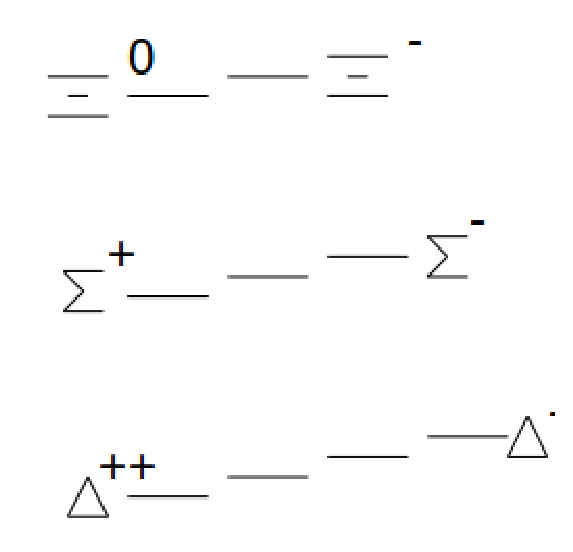
\includegraphics{p4}
\\
b. Since the observed particles split into three groups with an average energy difference of 150 between them, I would guess the energy of the 10th particle to be 1685.\\
c. We look for a 3D harmonic oscillator model with N=3 and approximately the right energy levels. 
We break the symmetry of the 3D harmonic oscillator by $\omega_1=\alpha,\ \omega_2=\omega_3=\beta$.
Setting $\alpha-\beta=150$ will create the desired separation between the energy levels.
To find the value of $\beta$ we calculate the lowest energy level $\braket{0 0 3}$ as $\frac{\beta+150}{2}+ \frac{1}{2}\beta + \frac{7}{2}\beta=1233$ so $\beta=257.33$.\\
d. The Hamiltonian for the 3D harmonic oscillator can be written using annihilation and creation operators:
\begin{gather}
 H=(a_1^\dagger a_1+\frac{1}{2})\hbar \omega_1+(a_2^\dagger a_2+a_3^\dagger a_3 + 1)\hbar \omega_{23}
\end{gather}
e. We find the best fit energies by varying our basic parameters and minimizing the mean-squared error (see p4.m).
With one million trials we find the best fit (in an MMSE sense) to be $\omega_1=408.07,\ \omega_2=258.78,\ \omega_3=256.27$.
With these parameters our prediction for the 10th particle is 1686.\\
f. We test the quality of the MMSE fit with a chi-squared test, incorporating the variance from the measurements.
We find a chi-squared value of 0.178 with 9 degrees of freedom, so we can reject the null hypothesis with confidence greater than 99.5% (our model is a good fit). 

\end{document}
